\todo[inline]{Explain the used metrics and how they relate to hypothesis}
\todo[inline]{Introduce the baselines, explain how they relate to the hypothesis, why they - are chosen, how they differ}
\todo[inline]{Explain methodology, why the chosen metric really captures the problem at - hand}
\todo[inline]{Work out differences of graph types, find similarities across datasets}
\todo[inline]{Provide the questions that are relevant for the hypothesis}
\todo[inline]{Answer these questions through metrics/results}

\todo[inline]{What is the best kernel for concept map classification?}
\todo[inline]{Extensions to WL?}


In order to test the hypothesis, we first derive a number of questions from the hypothesis.
We will also often compare the results on these questions for concept maps to co-occurrence graphs to find differences. While the comparison to co-occurrence graphs is interesting by itself, it is not entirely fair since co-occurrence graphs have far more nodes than concept maps.
Nevertheless, co-occurrence graphs capture the words of a text completely.

In the next chapter, we will give the results to the questions we posed in this chapter and also discuss their significance to the hypothesis.

\labelsubsection{Experiments}{subsec:experiments}
\todo[inline]{Test the hypothesis}
\todo[inline]{Tables with results}
\todo[inline]{Mention difficulties and possible solutions}
\todo[inline]{Add runtime analysis}

\subquestion{How diverse is the structure of the concept maps?}{question:structure_diversity}
When the structure of the graphs is mostly homogeneous or the structural differences are not distinct between graphs of different classes, the structure by itself will most likely not contribute to the classification performance.
When comparing the graph similarity under some graph kernel, the graphs of a given class should be distinguishable from the graphs of the other classes.

To explore the variance in the structure of concept maps, we look at the following metrics:
\begin{enumerate}
    \item{Histogram of the number of connected components}
    \item{Histogram of the size of connected components}
    \item{Average node/edge ratio}
\end{enumerate}

All these methods aim to find out the diversity of the connectedness of concept maps. There a lot of other metrics, but as we will see later on these metrics suffice to get a good picture about the structure of the concept maps.

\subquestion{How important is the structure of concept maps compared to the content?}{question:importance_structure}
Another important question is the relative importance of the structure compared to the content, or the labels.
For this we compare the results of different graph kernels that use \textbf{(a)} only content and \textbf{(b)} only structure and \textbf{(c)} both content and structure.

For the content-only kernel, we will simply count the number of occurrences of labels in the graphs and essentially create a bag-of-words representation of the graph. The kernel then creates the similarity score by calculating the inner product on these vector representations, effectively counting the number of common labels.

For the structure-only kernel, we will use a modified version of the Weisfeiler-Lehman kernel: before executing the WL kernel on the graphs, we first discard all labels on the graph. All nodes of all graphs get the same label. This way, only the structure gets used for the similarity score.

For the structure-and-content kernel, we use the plain Weisfeiler-Lehman graph kernel. We also added an extension to the kernel by using node weights as weights for the labels. We first extracted a weight for each node by calculating the node degree.
We added this extension to give additional weight to label matches of nodes with a greater number of neighbours, ie. higher degree, since matches with a greater neighbourhood are far less often.
Instead of the degree, one could also use another metric like PageRank and using the resulting node weights.

\todo[inline]{Using node weights is a trade-off: giving the nodes more weight when they are more connect implies that words that occur often have a high importance!}

\subquestion{How does the classification results of co-occurrence graphs compare to concept maps?}{question:comparison_coo}
For this question, we compare the classification results for concept maps and co-occurrence graphs. As noted before, this comparison is slightly unfair since co-occurrence graphs have far more content than concept maps.
Nevertheless, it is an interesting baseline for graph-based text-classification.

\subquestion{How does the classification performance with concept maps compare to non-structural, text-based approaches?}{question:comparison_text}
Here we test the classification performance of graph-based classification directly with the performance of text-only approaches.

\subquestion{How different are the datasets and how does it affect the classification performance?}{question:dataset_diversity}

\subquestion{How useful are the concept maps combined with text classification?}{question:comparison_combined}
When concept maps indeed have a structure that is useful for classification and which is not captured by text-only approaches, the classification performance should increase when combining graph- and text based approaches.
We test the performance of the combined text- and graph features by concatenating the vectors of both approaches and then training a classifier with these vectors.
We also compare the results with both text-only and graph-only approaches.

\subsubsection{Baselines}
\paragraph{Preprocessing}
Before creating the vector representations of the text documents or the creation of the co-occurrence graphs and concept maps, we first pre-process the plain text by

\begin{itemize}
\item{lowercasing the text,}
\item{removing non-printable characters,}
\item{replacing numbers with a \textit{NUMBER} placeholder,}
\item{replacing tabs and newlines with a space,}
\item{and normalizing the whitespace (eg. replacing multiple spaces with a single space)}
\end{itemize}
These pre-processing steps are similar to the pre-processing done in \cite{Cachopo2007}.

For the co-occurrence graphs, we also optionally filtered out the non-nouns to increase the compression and thus achieve more comparability to concept maps.

\paragraph{Text-based representations}
For the text classification pipeline, we used two different text vectorization algorithms, namely
\begin{itemize}
\item{Bag Of Words (BoW): this algorithm simply gathers all words in the corpus and creates a mapping between words and indices (ids). Then it creates a vector representation for each text so that the i-th vector component is the count of the corresponding word in the text. Ie. $i$ is the index of the word in the mapping.}
\item{Term-Frequency-Inverse-Document-Frequency (TfIdf): this approach is an extension to BoW. Instead of using only the counts of a word in the text, this approach also incorporates the term frequency and the inverse document frequency of the words into the vector representation.}
\end{itemize}
Both approaches can also be extended by not only utilizing single words (unigrams) but n-grams, too. A word n-gram consists of $n$ words that appear consecutively in the text.
For example, the sentence ``This is a sentence." has the following 2-grams, or bigrams: $\{ (This, is), (is, a), (a, sentence) \}$.
For our purposes, we looked at both uni-grams and bi-grams.
Note that word n-grams do not take word inversion into account, ie. the bigram (a, b) is not the same as (b, a).

\paragraph{Graph-based representations}
To compare the performance of concept maps with other graphs, we generated co-occurrence graphs with window sizes of $\{1, 2\}$.
We also evaluated the performance of co-occurrence graphs where only nouns are retained to mimic the compression factor of concept maps.

For the extraction of the concept maps from the text, we used the implementation by Falke \cite{Falke2017}.

\begin{figure}[ht]
\centering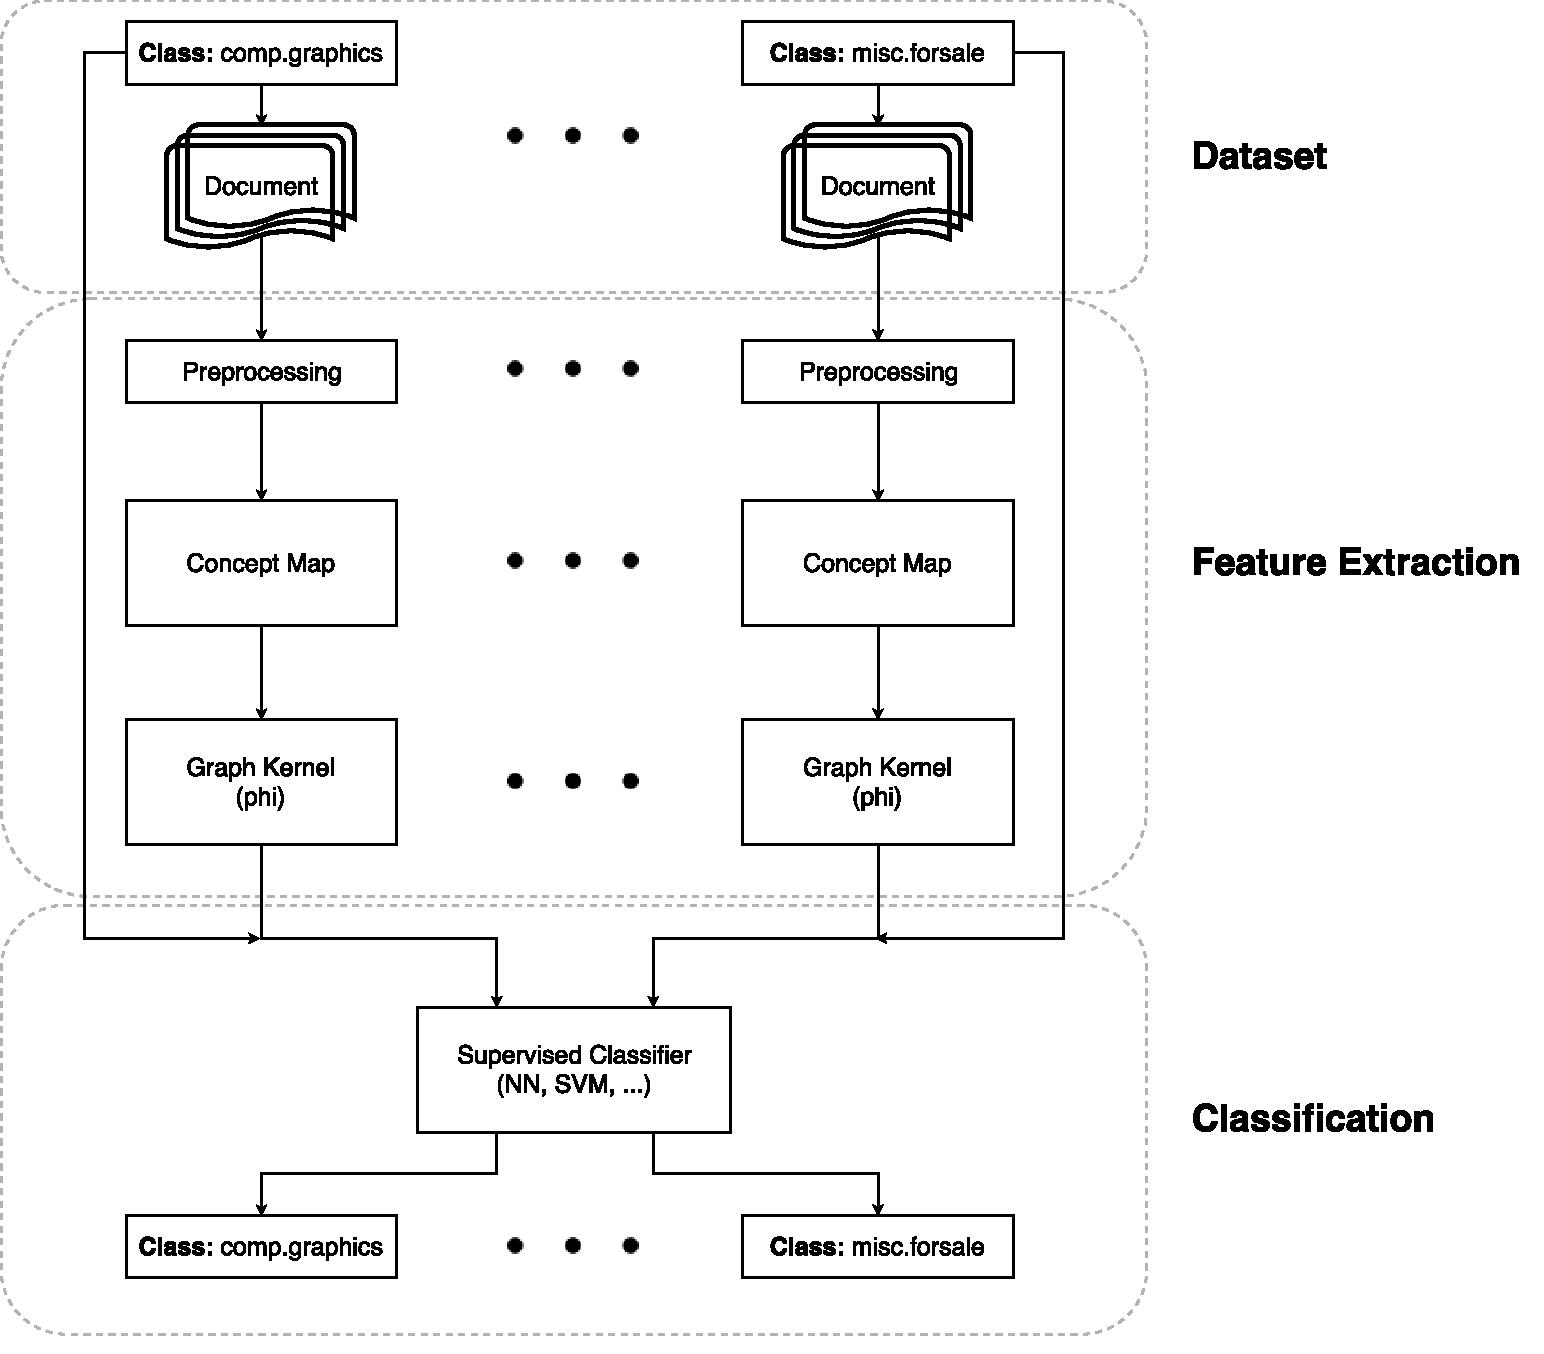
\includegraphics[width=0.6\linewidth]{assets/figures/approach.pdf}
\caption{Graph kernel based classification pipeline.}
\end{figure}
\todo[inline]{Add diagram for gram-matrix based classification.}

\labelsubsection{Datasets}{subsec:datasets}
\todo[inline]{A script to download all datasets is also provided alongside the other code}
\todo[inline]{What actually is different per dataset? Why these datasets?}

\paragraph{ling-spam}
The Ling-Spam dataset was created by Ion Androutsopoulos et al. \cite{Androutsopoulos2000}.
The corpus contains the texts that are categorized as ``spam" and ``no spam".
One thing to note is that the classification scores with standard methods are quite high by default, so most likely there is substantial increase in performance to be expected.

For this work, we used the version which can be downloaded from here \footnote{\url{http://csmining.org/index.php/ling-spam-datasets.html}}.


\paragraph{ng20}
The 20 Newsgroup corpus \cite{Lang} consists of posts from an internet forum. Each post is labeled with one of 20 different classes, corresponding to the topic it have been posted on. The texts are mostly informal and consist of discussions between users of the forum.
For this dataset, as an additional pre-processing step, we remove the headers and footers from the documents.

While the classes are nearly evenly distributed, some classes are highly correlated. This adds an additional difficulty to the task.
\todo[inline]{Cite!}

We obtained the ng20 dataset from here \footnote{\url{http://scikit-learn.org/stable/modules/generated/sklearn.datasets.fetch_20newsgroups.html#sklearn.datasets.fetch_20newsgroups}}.

\paragraph{reuters-21578}
This dataset has been collected and published by Carnegie Group, Inc. and Reuters, Ltd.

The class distribution of the reuters-21578 dataset is highly skewed, ie. the number of instances per class is not the same for all classes. 


We obtained the reuters-21578 dataset from here
\footnote{\url{http://www.nltk.org/book/ch02.html#reuters-corpus}}.


\paragraph{r8}
This dataset is a subset of the \textit{reuters-21578} dataset.
It consists of the 8 most frequent classes of the \textit{reuters-21578} dataset, ie. the 8 classes with the most documents.

\paragraph{review\_polarity}
\cite{Pang2004}.
\footnote{\url{http://www.cs.cornell.edu/people/pabo/movie-review-data/review_polarity.tar.gz}}

\paragraph{rotten\_imdb}
\cite{Pang2004}.
\footnote{\url{http://www.cs.cornell.edu/people/pabo/movie-review-data/rotten_imdb.tar.gz}}

\paragraph{tagmynews}
\footnote{\url{http://acube.di.unipi.it/repo/news.gz}}

\paragraph{webkb}
\footnote{\url{http://www.cs.cmu.edu/afs/cs/project/theo-20/www/data/}}

\begin{figure}[ht]
\centering
\begin{tabular}{lrrrr}
{} &  \# classes &  \# docs &  median \#words/doc &  \#uniq. words/\#words \\
\midrule
ling-spam       & 2 & 2893 & 277 & 0.20 \\
ng20            & 20 & 18846 & 79 & 0.07 \\
reuters-21578   & 90 & 13328 & 94 & 0.07 \\
review\_polarity & 2 & 2000 & 589 & 0.16 \\
rotten\_imdb     & 2 & 10000 & 19 & 0.34 \\
tagmynews       & 7 & 32600 & 24 & 0.11 \\
webkb           & 7 & 8274 & 158 & 0.15 \\
\bottomrule
\end{tabular}
\caption{Dataset statistics.}
\end{figure}

\labelsubsection{Methods}{subsec:methods}

\subsubsection{Cross-Validation}
For all the classification tasks we used train-/validation- and test sets.
The split is done as follows: 85\% for train- and validation set together and 15\% for the validation set.
We then use stratified k-fold cross-validation to further split the train- and validation set. In our case, we used $k = 3$, meaning that $\frac{2}{3}$ of the dataset is used for training, and the rest for validation.
The stratification ensures that the class distribution in the train set is (nearly) the same as in the validation set.

\todo[inline]{Hold-out set!}

\subsubsection{Metrics}
We evaluated a number of metrics for each classification task, namely: 
recall, precision, accuracy and the F1-score. We mostly focus on the F1-score since it captures the overall performance of classification algorithms.

\subsubsection{Significance tests}
When comparing two models we used the permutation test, or exact test, to test the significance of the difference in performance of these two approaches.
The permutation test tests whether the observed difference of the performances of the two approaches is the product of chance.
The test only returns a probability for observing a given performance difference. The test does not give a definite answer whether the difference was due to chance.
When the probability of observing the difference by chance is below a given threshold, we say that the test shows that the approaches really differ in their performance.

Following is an example of a permutation test.

\paragraph{Example}
In this example we will use the permutation test to test whether the 
  performances of two given classifiers, Model A and B, differ in a non-random way.
In Figure \ref{fig:example_permutation_test} we depicted the steps in the permutation test. 
In our example, the hypothesis is that Model A has a lower performance than Model B.
For this example we chose accuracy as the score metric.
To calculate the accuracy, we need the true labels of the dataset, seen in Figure \ref{fig:example_permutation_test} \textbf{\subref{fig:permutation_test_true}}.
In Figure \ref{fig:example_permutation_test} \textbf{\subref{fig:permutation_test_model_predictions}} we see the predicted labels of the two models and the accuracy as a score beneath them. 
We also see the difference in the scores.
In Figure \ref{fig:example_permutation_test} \textbf{\subref{fig:permutation_test_model_predictions}} we also see that Model A has a lower score than Model B.
This lower score could be due to chance and not because Model B is fundamentally better than Model A.
To test our hypothesis more throughly we now execute the permutation test.
In the first step, Figure \ref{fig:example_permutation_test} \textbf{\subref{fig:permutation_test_samples}}, we generate $n$ samples by interchanging the predictions of the two models randomly.
Here, we depicted three randomly selected samples from the $n$ generated samples.
To generate a sample, we switch the predictions of Model A and B for every document with a probability of 0.5.
The switch of two predictions is marked with a red arrow in our depiction.
In the optimal case, one could generate all possible permutations of the predictions, ie. generate all possible samples.
Unfortunately this often is not an option due to the sheer number of possibilities. That said, generating a large number of samples also gives a good basis for judgment.
In the next step, we calculate the accuracy scores for both models for each of the $n$ samples and also calculate the difference between these scores.
In Figure \ref{fig:example_permutation_test} \textbf{\subref{fig:permutation_test_distribution}} we see the histogram of score differences in the samples.
The red lines mark the initially observed difference between the models A and B (also it's negative).
In the last step, we gather these differences and count the number of samples, $n_{higher}$, where the absolute difference between the models is smaller than the score difference of the original predictions of Model A and B.
$n_{higher}$ divided by the total number of generated samples, $n$, is then the frequency of samples, $f_{higher} = \frac{n_{higher}}{n}$, where the score difference was higher when randomly exchanging the predictions compared to the original observed score difference.
$f_{higher}$ gives an intuition about the likelihood of observing the difference between the scores of Model A and B.
In the histogram of observed differences Figure \ref{fig:example_permutation_test} \textbf{\subref{fig:permutation_test_distribution}} this $f_{higher}$ corresponds to the ratio between the area of elements in the blue surface to total area of the histogram.
In our example, $f_{higher}$ is 0.135, meaning that the probability to observe the score difference we see between the two models is 13.5\% when randomly exchanging the predictions of the two models.
This is far too high to accept the hypothesis on ground of these predictions.

\todo[inline]{What confidence interval did we choose?}
\todo[inline]{\url{https://stats.stackexchange.com/questions/104040/resampling-simulation-methods-monte-carlo-bootstrapping-jackknifing-cross}}

\begin{figure}[ht]
  \subfloat[True labels]{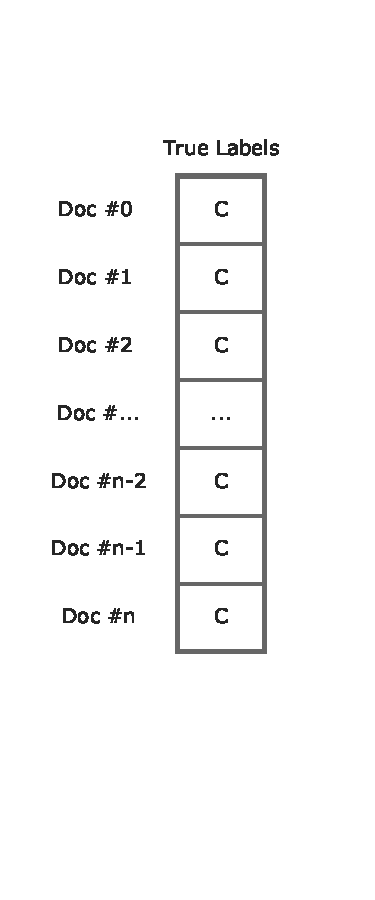
\includegraphics[width=0.19\textwidth]{assets/figures/permutation_test/true_labels.pdf}\label{fig:permutation_test_true}}
  \hfill
  \subfloat[Predictions]{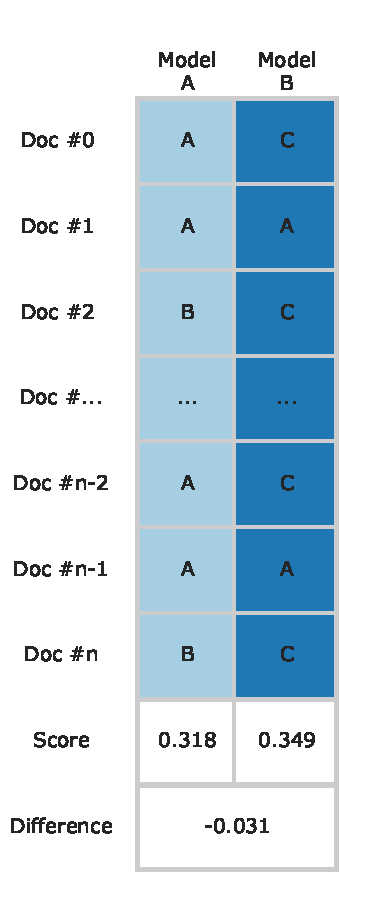
\includegraphics[width=0.17\textwidth]{assets/figures/permutation_test/initial_predictions.pdf}\label{fig:permutation_test_model_predictions}}
  \hfill
  \subfloat[Samples]{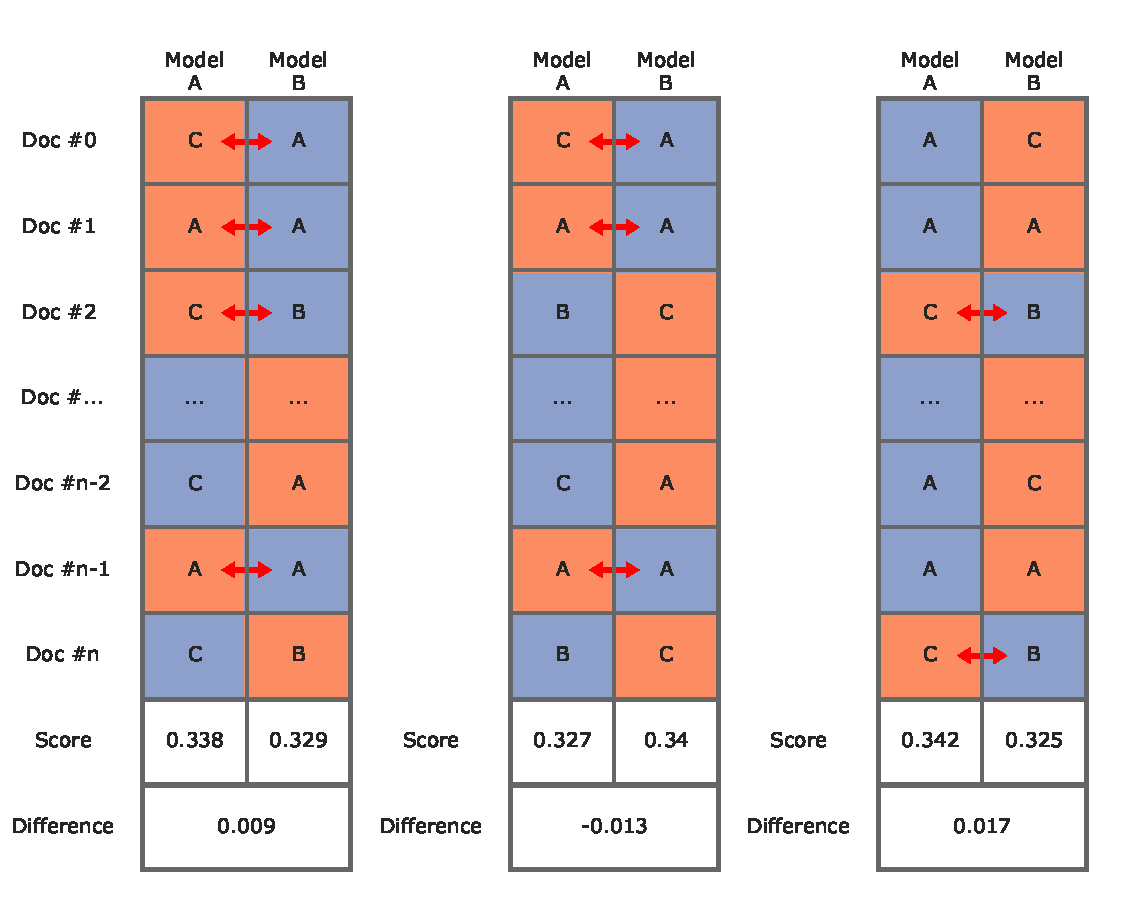
\includegraphics[width=0.51\textwidth]{assets/figures/permutation_test/samples.pdf}\label{fig:permutation_test_samples}}
  \\
  \subfloat[Observed differences in sample scores]{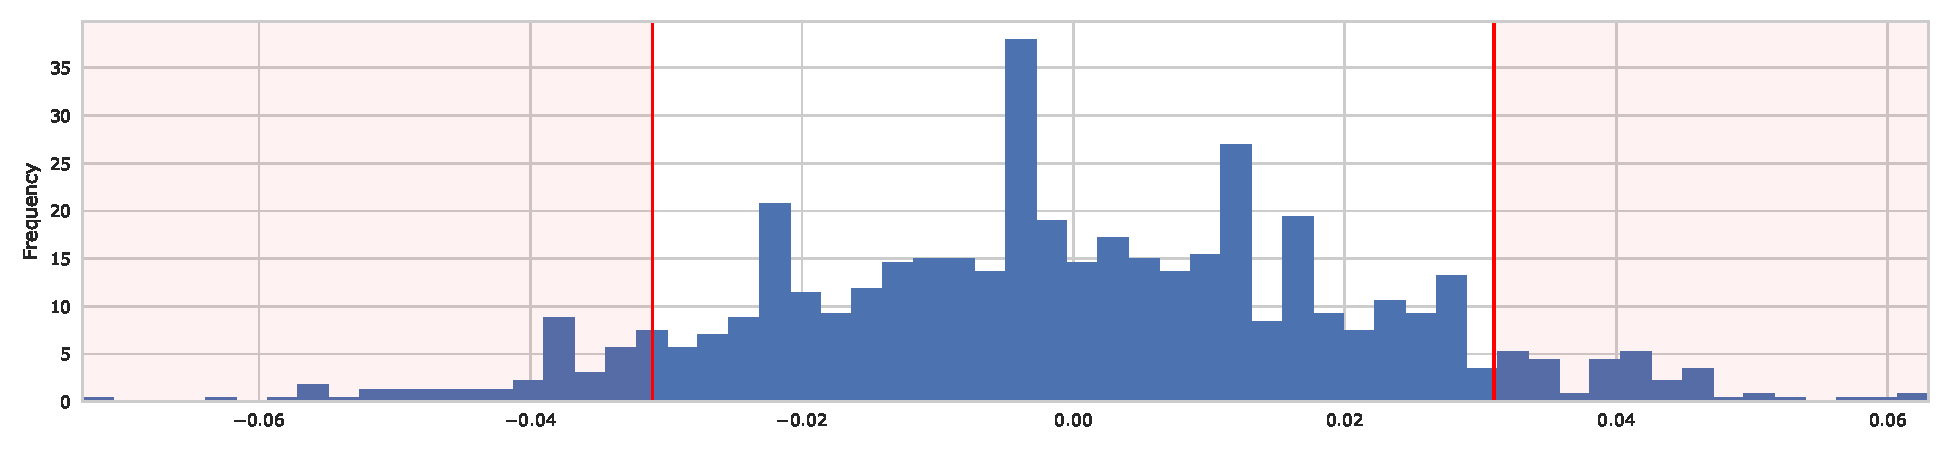
\includegraphics[width=1\textwidth]{assets/figures/permutation_test/distribution.pdf}\label{fig:permutation_test_distribution}}
  \caption{Permutation test example. A significance test is most often used to test whether a hypothesis is true with a given confidence.}
  \label{fig:example_permutation_test}
\end{figure}


\labelsubsection{Implementation}{sec:implementation}
For the implementation of all these experiments, we used mostly Python.
\todo[inline]{Scikit-learn, networkx, \dots}
\todo[inline]{Code by Tobias to extract concept maps}
